%%% Template for AUTHOR's DRAFT paper in FCAA, WITHOUT Journal's head
%%% created Nov. 28, 2010 by V. Kiryakova
%%% uses "fcaa.cls", as modification of "amsart.cls" for the FCAA style,
%%% and auxiliary file "fcaa_style.tex" stating page margins, fontsize, defs for theorems, proofs etc.
%%% Put the files "fcaa.cls" and "fcaa_style.tex" in same directory

 \documentclass[twoside,reqno,11pt]{fcaa}
 \input fcaa_style

 \usepackage{hyperref} % Editor will use to create hyperlinks

% to have 2-digits numbering for equation, use:
 \def\theequation{\arabic{section}.\arabic{equation}}

%%%%%%  First page footnote for Copyright and Springer logo
 \def\themycopyrightfootnote{\vspace*{3pt}
 \copyright \, Year\,  Diogenes  Co., Sofia
   \par  \noindent pp. xxx--xxx
   \hfill  \vspace*{-36pt}
   % \mbox{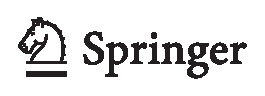
\includegraphics[scale=0.65]{springer.eps}}
  }
%%%%%%%%%%%%%%%%%%%%%%%%%%%%%%%%%%%%%%%%%%%%%%%%%%%%%%%%%%%%

  \setcounter{page}{1}
  \thispagestyle{empty}

%%%%%%%%%%%%%%% begin make title %%%%%%%%%%%%%%

 %%% TITLE: texts in [.] is abbreviated (1st line) title for running heads
 %%% Author(s): put in brackets [.] the short author's name

 \title[TITLE OF PAPER \dots]{TITLE OF PAPER \\ [4pt] IN ``FCAA'' JOURNAL}
 \author[V. Kiryakova, S. Author]{Virginia Kiryakova $^1$, Second Author $^2$}

%%%%%%%%%%%%%%%%%%%%%%%%%%%%%%%%%%%%%%%%%%%%%%%%%%%%%%%%%%%%%%%%%%%%%%%
                    % THE BEGINNING %
 \begin{document}

 \vbox to 2.5cm { \vfill }

%%% to make empty space of approx. 2.5cm %%%%%%
%%% will be replaced by Editor with the journal's and Versita logos %%%%%%%%

 \bigskip \medskip

%%%% Abstract %%%%%%%%%%%%%%%%%%%%%%%%%
 \begin{abstract}

Text of the abstract. Text of the abstract. Text of the abstract.
Text of the abstract. Text of the abstract. Text of the abstract.
Text of the abstract. It should give a comprehensive idea about the
paper's subject and the author's results. This Abstract will be
available free on SpringerLink.

 \medskip

{\it MSC 2010\/}: Primary 26A33: Secondary 33E12, 34A08, 34K37,
35R11, 60G22, ...

 \smallskip

{\it Key Words and Phrases}: fractional calculus, Mittag-Leffler
type functions, fractional ordinary and partial differential
equations, ...

 \end{abstract}

 \maketitle

%%%%%%% end make title %%%%%%%%%%%%%%%%%%%%%%%%%%%%%%%%%%
 \vspace*{-16pt}

%%%%%%%% begin papers' body %%%%%%%%%%%%%%%%%%%%%%%%%%%%%

%%%%%%%%%%%%%%%%%%%%%%%%%%% Section 1 %%%%%%%%%%%%%
%\section{Introduction}\label{Sec:1}

 \section{First section of the paper}\label{sec:1}

\setcounter{section}{1}
\setcounter{equation}{0}\setcounter{theorem}{0}


Text ... (for details, see \cite{GasRah}, \cite{Rosbl}, \cite{Kir},
\cite{Moak}) ...

%%%% example of definition %%%%
 \begin{definition}\label{Def3}
Text of Definition~\ref{Def3}.
 \end{definition}

   \vspace*{-12pt} %%% example of subsection:
 \subsection{Preliminary results}\label{subsec:1.1}

%%%% example of theorem %%%%%%%%%%
 \begin{theorem}\label{Th1}
Text of Theorem~\ref{Th1} ....
 \end{theorem}

 \proof %%%%%%%%%%%%%
 Give here the proof of Theorem~\ref{Th1}. Example for
equation:
\begin{equation}\label{eq1}
ax^2+bx +c =0.
\end{equation}
 As seen by equation \eqref{eq1}, it is ...
 The proof follows from Ref. \cite{Moak}.
 \proofend %%%%%%%%%%

%%%% example of corollary %%%%
 \begin{corollary}\label{Cor2}
Text of Corollary~\ref{Cor2}.
 \end{corollary}

 \proof
 Here comes the proof of Corollary~\ref{Cor2}.
 \proofend

%%%%%%%%%%%%%%%%%%%%%%%%%%%%%%%%%%%%%%%%%%%%%%%%%%
\section{Second section of the paper}\label{sec:2}

\setcounter{section}{2}
\setcounter{equation}{0}\setcounter{theorem}{0}


 Text ... As seen in Section~\ref{sec:1}, the equation
(\ref{eq1}), $ a\neq 0$, has the solutions
 \begin{equation}\label{eq2}
 x_{1,2}= {\frac {-b \pm \sqrt{b^2-4ac}}{2a}}\,.
 \end{equation}

 %%% example of examples %%%%%
 \begin{example}\label{Ex1}
 Let us take in (\ref{eq2}) ... Then, by Theorem~\ref{Th1}, ...
 \end{example}

 \begin{example}\label{Ex2}
 Under same conditions as in Example~\ref{Ex1}, we consider ...
 \end{example}

%%%%%%%%% example for figure %%%%%%%%%%%%%%%%%%%
 \begin{center}
 
\includegraphics[scale=0.4]{versita.eps}
 \hspace*{2cm}
 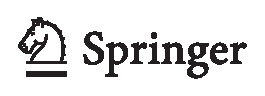
\includegraphics[scale=0.7]{springer.eps}

 \bigskip

Fig. 2.1: The logos of the co-publishers of the journal
 \end{center}
%%%%%%%%%%%%%%%%%%%%%%%%%%%%%%%%%%%%%%%%%%%%%%%

\smallskip
%%%%%%%%%%%%%%%%%%%%%%%%%%%%%%%%%%%%%%%%%%%%%%%%%
\section*{Acknowledgements}

The author thanks his institution for the support, under Grant No
...

%%%%%%%%%% References %%%%%%%%%%%%%%%%%%%%%%%%%%%%%%%%
%%%% arranged in ALPHABETIC ORDER of Authors' Families

 \begin{thebibliography}{99}
 \normalsize

%%%% example for a book %%%%%%%%%%%%%
\bibitem{GasRah}
 G. Gasper, M. Rahman,
 {\it Basic Hypergeometric Series}.
 Cambridge University Press, Cambridge (1990).

%%%% example for article in FCAA journal %%%%%%%%%%%%%%%%%
\bibitem{Kir}
 V. Kiryakova,
 A brief story about the operators of generalized
fractional calculus.
 \emph{Fract. Calc. Appl. Anal.} \textbf{11}, No 2 (2008), 201-218.

%%%% example for journal's article %%%%%%%%%%%%%%%%%
\bibitem{Moak}
 D.S. Moak,
 The $q$-analogue of the Laguerre polynomials.
{\it J. Math. Anal. Appl.} {\bf 81}, No 1 (1981), 20-47.

%%%% example for a paper in Proceedings %%%%%%%%%%%%%
\bibitem{Rosbl}
 M. Rosenblum,
 Generalized Hermite polynomials and the Bose-like oscillator
 calculus.
 In: {\it Operator Theory: Advances and Applications},
 Birkh\"auser, Basel (1994), 369-396.
%%%%%%%%%%%%%%%%%%%%%%%%%%%%%%%%%%%%%%%%%%%%%%%%%%%%

\end{thebibliography} %%%%%%%%%%%%%%%%%%%%%%%%%%%%%%%%

%%%%%%%%%% put authors' addresses here, in \it %%%%%%%%

 \bigskip \smallskip

 \it

 \noindent
%(First) Author's full postal address
$^1$ Institute of Mathematics and Informatics \\
Bulgarian Academy of Sciences \\
"Acad. G. Bontchev" Str., Block 8 \\
Sofia -- 1113, BULGARIA  \\[4pt]
e-mail: virginia@diogenes.bg
\hfill Received: November 28, 2010 \\[12pt]
% Second Author's address
$^2$ Dept. of Physics, University of Bologna\\
Via Irnerio 46, I -- 40126 Bologna, ITALY \\[4pt]
e-mail: .....

\end{document} %%%%%%%%%%%%%%%%%%%%%%%%%%%%%%%%%%%%%
